%--------------------------------------------------------------
\section{Design do projeto}
%--------------------------------------------------------------
Cogitando a missão do projeto, surgiu a ideia de dar o nome \gls{ifriends} para o sistema, cuja origem é a junção de duas palavras: IF e \textsl{friends}. Isto devido a elas retratarem bem o âmbito que será atingido, já que tais palavras em conjunto transmitem o significado de ``amigos do \acs{ifsp}'', nome ideal para um projeto que visa tornar a interação dos alunos mais favorável.

A próxima etapa do desenvolvimento inicial da marca foi a elaboração de uma logo, assim como a definição das cores iniciais do sistema. A logo foi desenvolvida por meio do \gls{canva}, pois a plataforma se encontrava nos intermédios necessários para a elaboração da mesma. 

\begin{figure}[htb]
\centering
\caption{Logo do projeto}
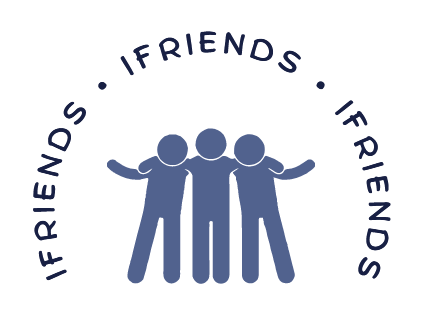
\includegraphics[width=0.3\textwidth]{anexos/Imagens_Proposta/logo.png}
\fonte{Os autores}
\end{figure}
\FloatBarrier

Já a seleção das cores iniciais do sistema traçou um caminho através de um estudo a respeito da psicologia das cores, visto que a equipe se preocupou em passar uma boa experiência até mesmo no quesito visual. Dessa forma, se definiu o azul e suas variações como a cor principal do sistema, já que segundo \citeonline{Tornos2021Sep}, os tons de azul se associam a princípios como: proteção, tranquilidade, fidelidade, compromisso, verdade, estabilidade, criatividade, entre outros. Vale ressaltar que o sistema ainda contará com outras cores, como roxo e algumas de suas variações, cores de sistema: variações de verde e vermelho, e cores neutras: variações de preto, cinza e branco.

Ainda, outro ponto considerado na criação da proposta foi a experiência do usuário final, pois mostrado assim como na \autoref{pesquisa}, a equipe se preocupou em estudar e conhecer melhor as dores deles. Visto que, segundo \citeonline{BibEntry2020Aug}, para tornar essa experiência agradável o sistema deve recorrer aos requisitos do modelo de colmeia desenvolvido por Peter Morville, sendo eles: útil, utilizável, desejável, acessível, confiável, localizável e valioso, conforme observado na \autoref{modelo colmeia}.

\begin{figure}[htb]
\centering
\caption{\label{modelo colmeia} Modelo Colmeia}
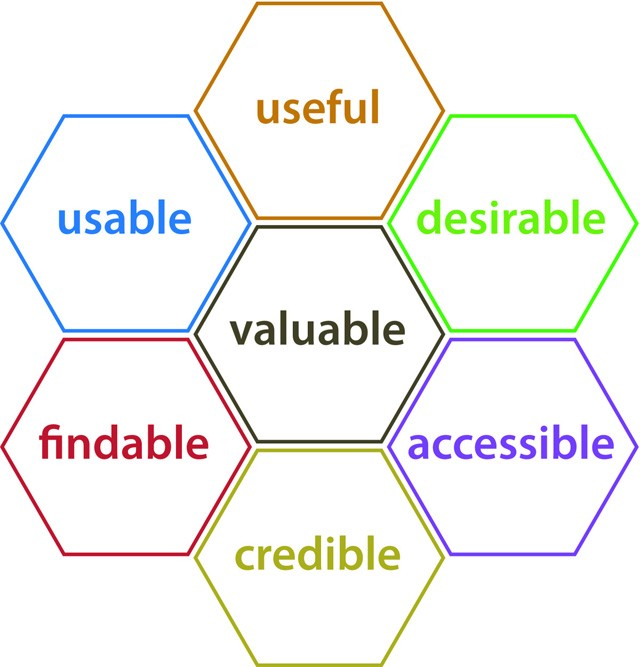
\includegraphics[width=0.3\textwidth]{anexos/Imagens_Proposta/modelo_colmeia.jpg}
\fonte{liferay.com}
\end{figure}
\FloatBarrier

% -------------------------------------------------------------
\subsection{Prototipagem}
% -------------------------------------------------------------
Para a prototipação se considerou os apontamentos de \citeonline{ferreira:2020} qual considera que ``prototipar é trazer, para o mundo real, o mundo palpável, as ideias de negócio construídas no mundo abstrato, na teoria''. Isto é, o autor comenta que um protótipo é um recurso utilizado para demonstrar e escolher a solução para representar uma ideia, podendo ser efetuado com entregas digitais, como telas de sistema. Dado isto, a próxima seção apresentará as telas prototipadas do projeto de sistema \gls{ifriends}.

Ainda, para auxiliar na prototipação das telas, foi elaborado um mapa mental de modo a representar melhor o fluxo do nosso projeto, que pode ser conferido na \autoref{Fluxo da aplicação}.

\begin{figure}[htb]
\centering
\caption{\label{Fluxo da aplicação} Fluxo da aplicação}
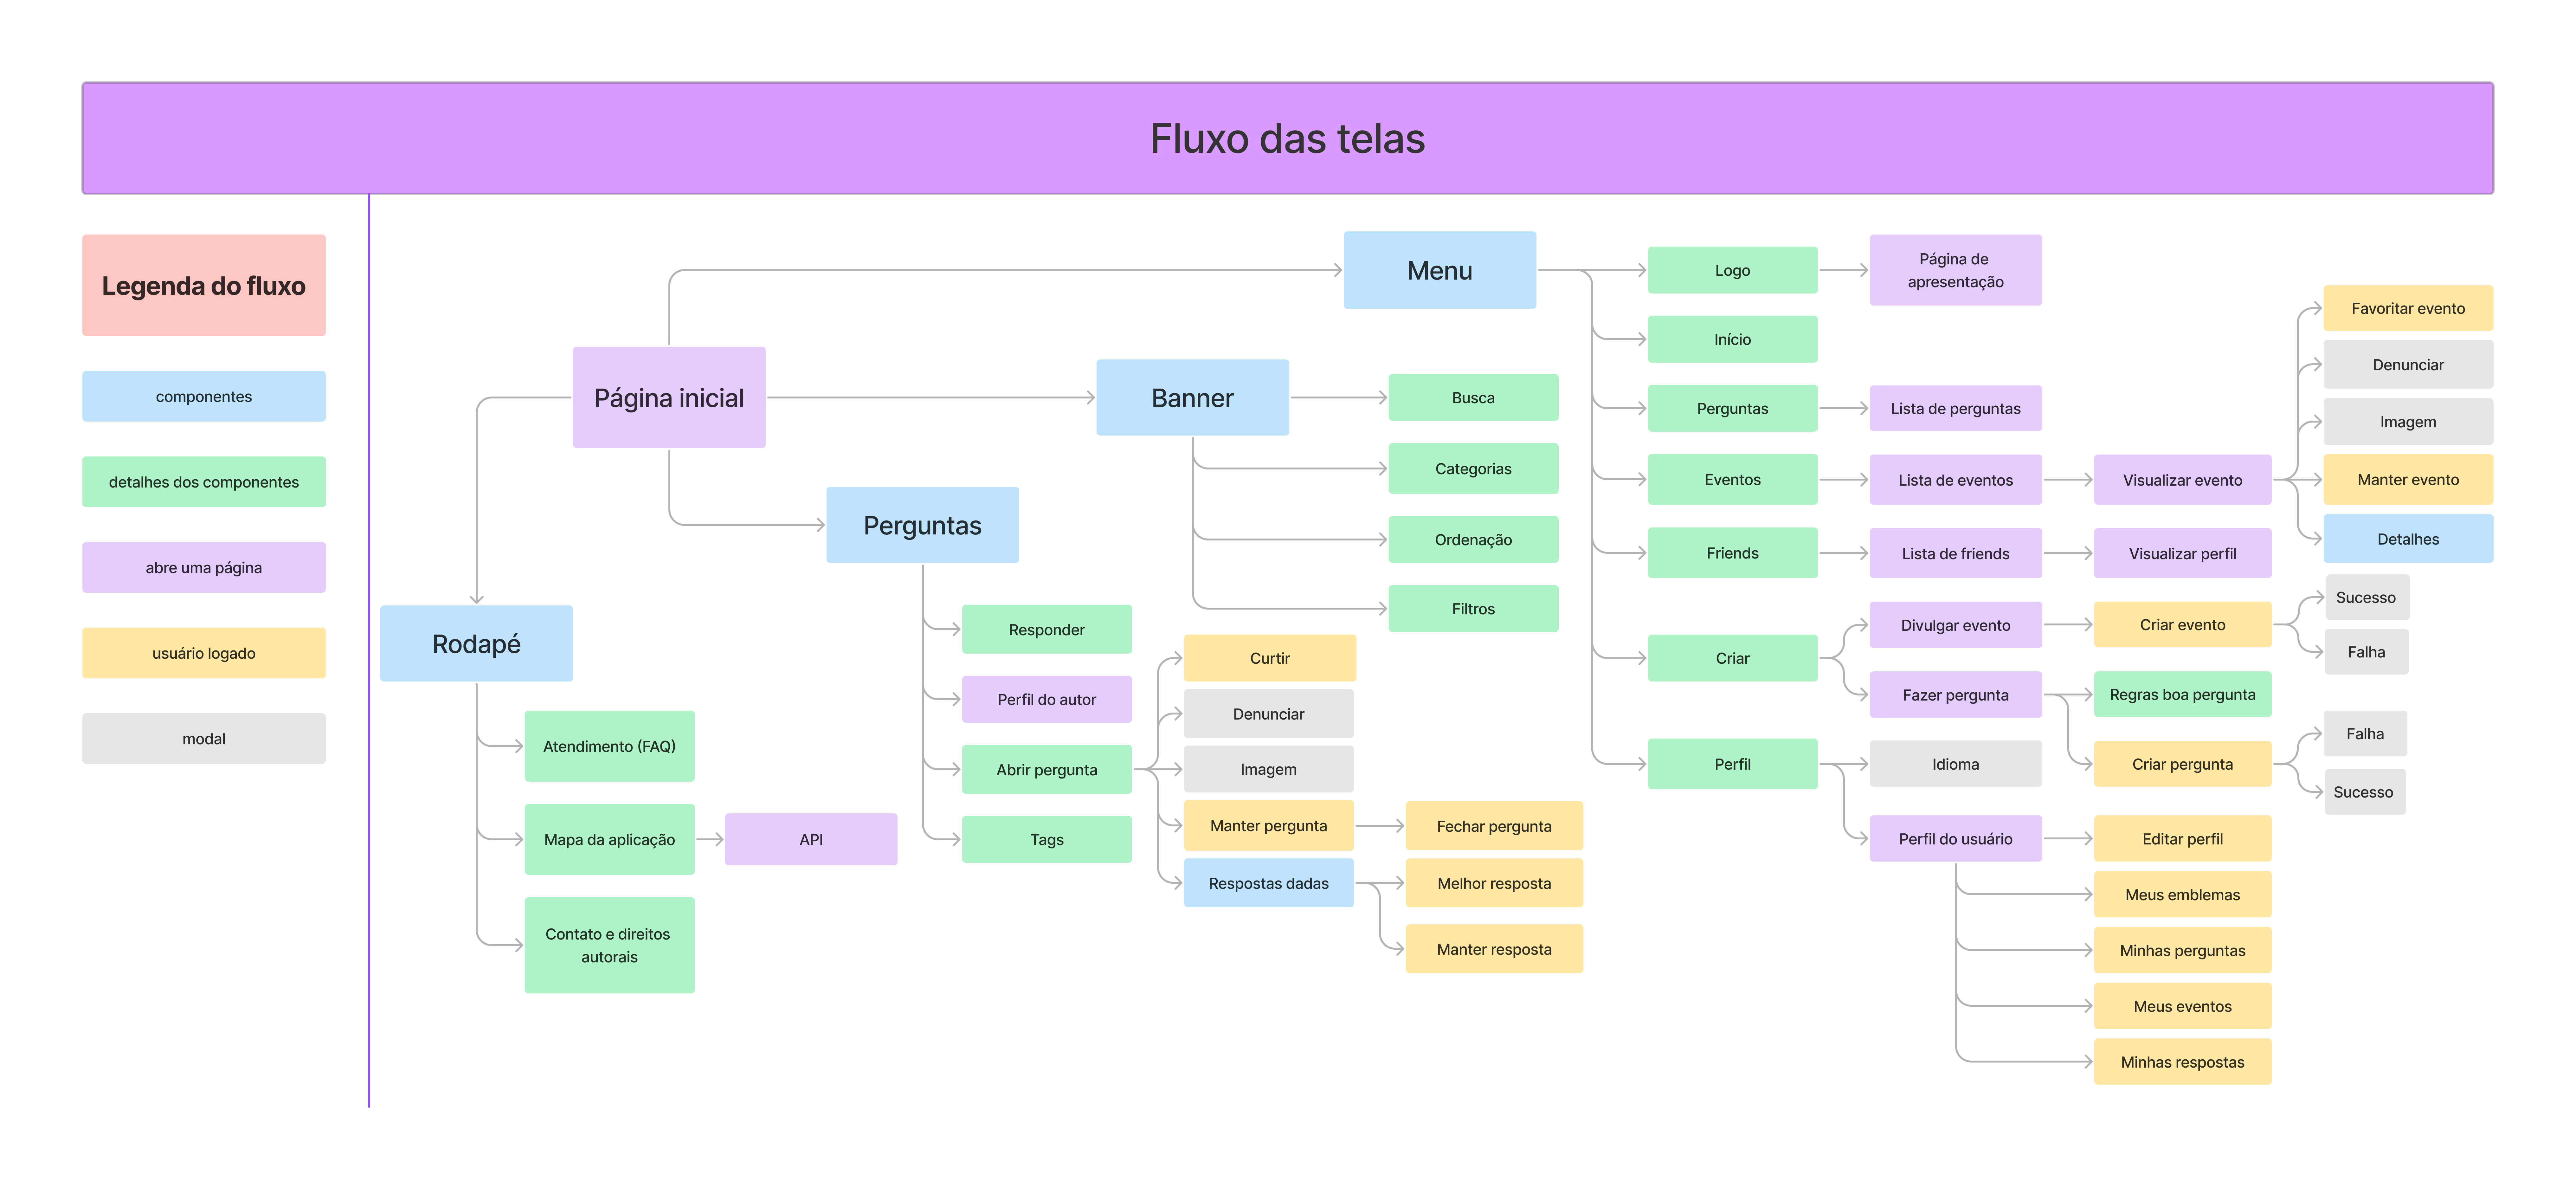
\includegraphics[width=1\textwidth]{anexos/Imagens_Prototipo/fluxo_telas.png}
\fonte{Os autores}
\end{figure}
\FloatBarrier

% -------------------------------------------------------------
\subsubsection{Protótipos de alta fidelidade}
% -------------------------------------------------------------
As figuras referentes a prototipagem de alta fidelidade podem ser encontradas no \autoref{prototipação}, onde cada tela apresenta uma breve contextualização sobre o seu conteúdo. De todo modo, a apresentação pode ser visualizada também pelo \href{https://www.figma.com/proto/GhIlybDubGmr3NkRU0a9GP/Protótipo---IFriends?node-id=73\%3A321}{Figma}.
